\section{Euclidean Voronoi Diagrams}
In this section we focus on proving some properties of the Voronoi diagram when the norm is the Euclidean norm, that is $\norm{\,\cdot\,}_2$. Here is the example from earlier:
\begin{figure}[H]
    \centering
    \subfloat{
      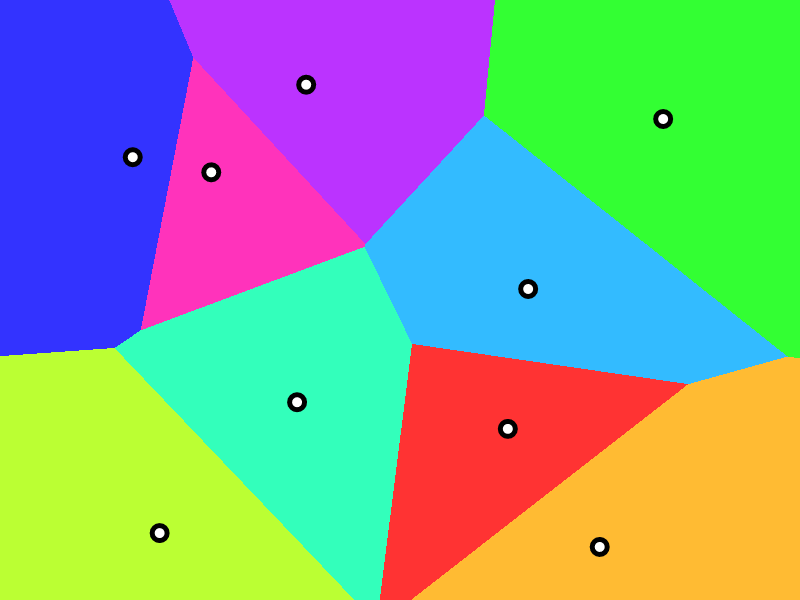
\includegraphics[scale=0.21]{naive-voronoi-L2}
    }
    \subfloat{
      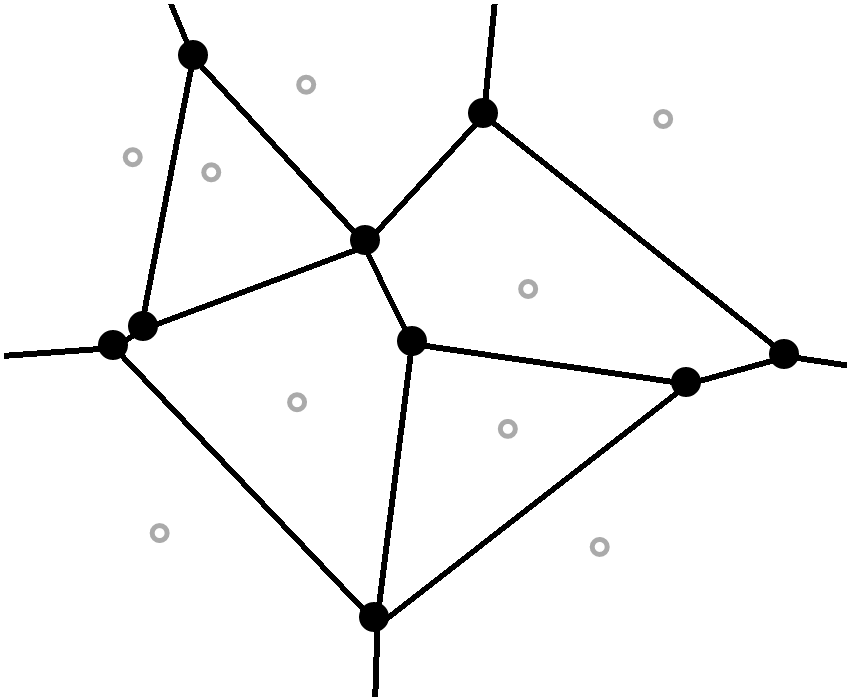
\includegraphics[scale=0.18]{naive-voronoi-graph-L2}
    }
\end{figure}
From linear algebra we know that $\norm{v}_2 = \sqrt{\ip{v}{v}}$, where $\ip{\,\cdot\,}{\,\cdot\,}$ is the usual dot product on $\R^2$. Given two points $p, q \in \R^2$ then the \textbf{bisector} of $p$ and $q$ is denoted by $\bi(p, q) \subset \R^2$ and denotes the set of points on a line $\ell$ which passes through the midpoint of $p$ and $q$ and is orthogonal (w.r.t. $\ip{\,\cdot\,}{\,\cdot\,}$) to the vector $p - q$.
\[
    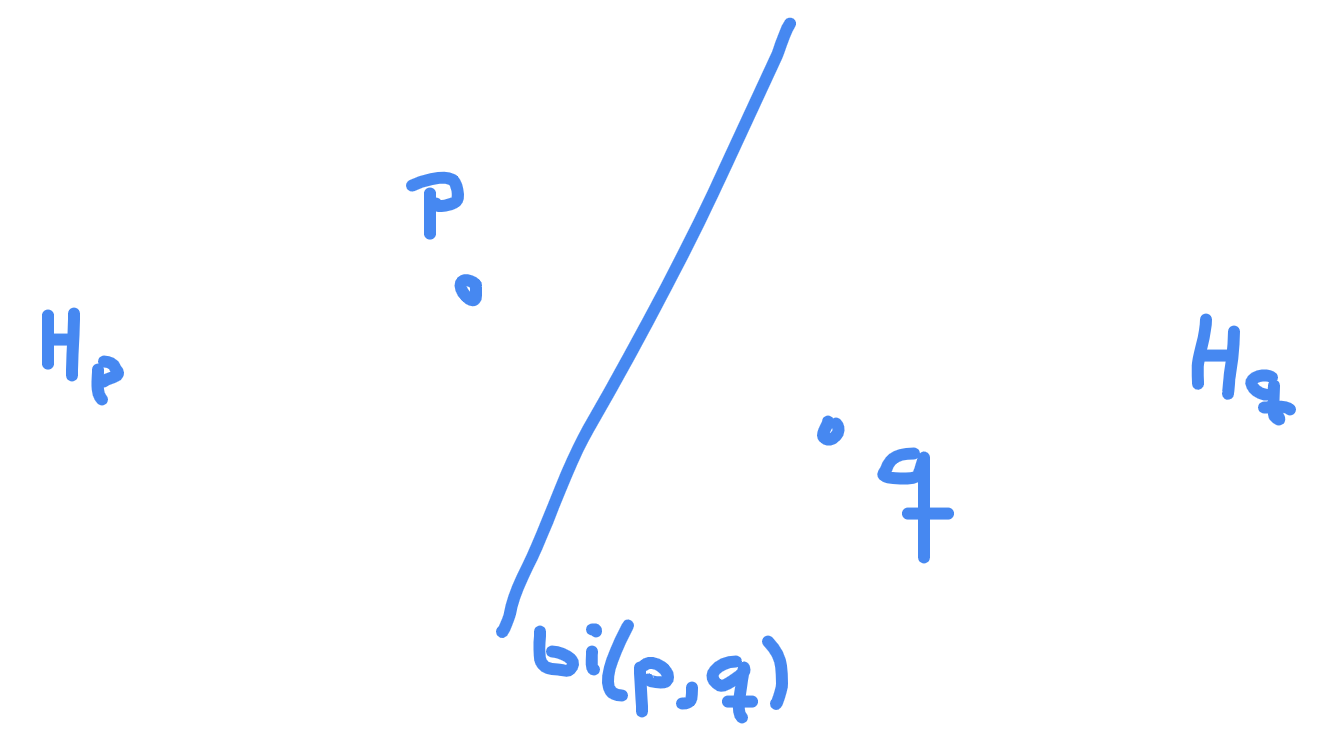
\includegraphics[scale=0.22]{temp-fig-2}
\]
A bisector $\bi(p, q)$ splits the plane into two \textbf{half-planes} $H_p$ and $H_q$ such that $p \in H_p$ and $q \in H_q$. We define $h(p, q)$ to be the open half-plane which contains $p$, that is the interior of $H_p$. So we have that
\[
    \R^2 = h(p, q) \cup \bi(p, q) \cup h(q, p).
\]
\begin{prop} \label{prop:hyperplaneinclusionproperty}
$r \in h(p, q)$ if and only if $\dist(r, p) < \dist(r, q)$.
\end{prop}
\begin{proof}
\[
    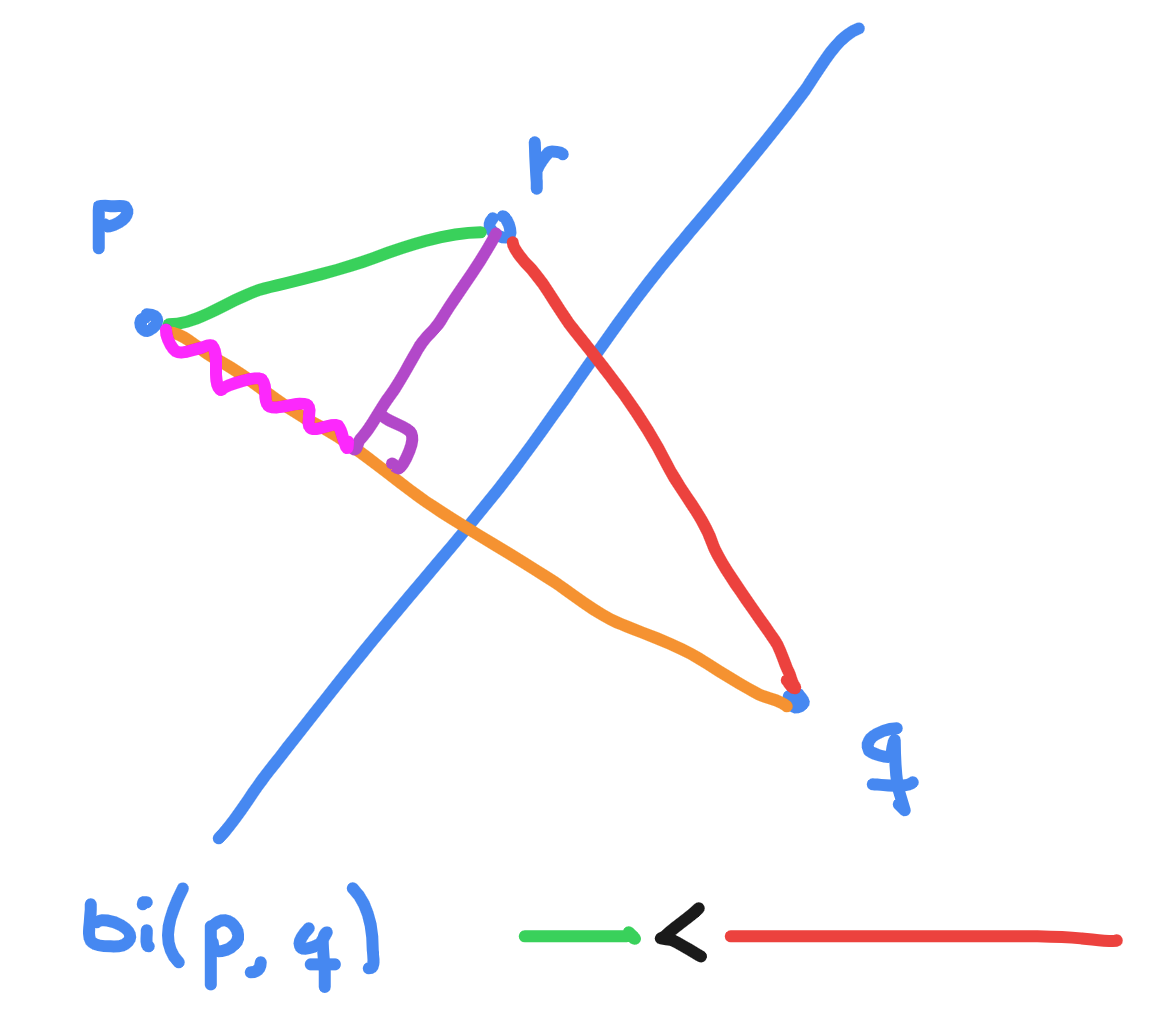
\includegraphics[scale=0.25]{temp-fig-1}
\]
\todo{Formalize} Proof sketch: We want to project $r$ onto the orange line. As long as $r \in H_p$ then the squiggly pink segment is shorter than the orange segment, which will make the green segment shorter than the red segment (which is what we want to show).
\end{proof}

\begin{cor} \label{prop:cellsareintersectionsofhalfplanes}
For every Voronoi cell we have
\[
    \mathcal{V}(p_i) = \bigcap_{\substack{1 \leq j \leq n \\ j \ne i}} h(p_i, p_j).
\]
\end{cor}
\begin{proof}
``$\subset$'': Let $r \in \mathcal{V}(p_i)$. Then $\dist(r, p_i) < \dist(r, p_j)$ for all $i \ne j$. Prop \ref{prop:hyperplaneinclusionproperty} then gives us that this is equivalent to $r \in h(p_i, p_j)$ for all $i \ne j$.

``$\supset$'': This argument is symmetrical to the above argument.
\end{proof}
A Voronoi cell is thus the intersection of convex sets and is therefore convex. We conclude that the Voronoi cells are open and convex (possibly unbounded) polygons with at most $n - 1$ vertices and $n - 1$ edges. \\

We now look at the shape of the entire Voronoi diagram. From Corollary \ref{prop:cellsareintersectionsofhalfplanes} it follows that the edges of $\VorG(P)$ are made up of parts of straight lines, namely the bisectors between different points of $P$. We now classify these based on the structure of the points in $P$:
\begin{thm} \label{prop:structureofentirevoronoidiagram}
If the points in $P$ are collinear then $\VorG(P)$ consists of $n - 1$ parallel lines. Otherwise, $\VorG(P)$ is connected and its edges are either segments or half-lines.
\end{thm}
\begin{proof}
Assume that the points in $P$ are collinear. By applying an isometry to $P$, we may assume without loss of generality that the points of $P$ lie on the $x$-axis:
\[
    P = \curly{(x_1, 0), (x_2, 0), \ldots, (x_n, 0)},
\]
where we assume that $x_1 < x_2 < \cdots < x_n$ by rearranging the points if necessary. See the proof of Theorem \ref{thm:voronoicansort} for a visualization of $\Vor(P)$. By definition, we have that $p \in \VorG(P)$ if and only if $p \not\in \mathcal{V}(x_i, 0)$ for all $i$. Let $(x, y) \in \R^2$ such that $x_i < x < x_{i+1}$. Then $(x, y) \in \VorG(P)$ if
\[
    \dist((x, y), (x_i, 0)) = \dist((x, y), (x_{i+1}, 0)).
\]
If furthermore $(x, y) \in \VorG(P)$ then we get
\begin{align*}
    &\norm{(x, y) - (x_i, 0)} = \norm{(x, y) - (x_{i+1}, 0)} \\
    \iff &\sqrt{(x - x_i)^2 + y^2} = \sqrt{(x - x_{i+1})^2 + y^2} \\
    \iff &\abs{x - x_i} = \abs{x - x_{i+1}}.
\end{align*}
Thus if $(x, 0) \in \VorG(P)$ then $(x, y) \in \VorG(P)$ for all $y \in \R$. This shows that $\bi((x_i, 0), (x_{i+1}, 0)) \subset \VorG(P)$ for all $i < n$. Every point of $\VorG(P)$ is on one of these bisectors, and the bisectors are all parallel, which proves the claim. \todo{Clean up above argument and consider if anything is missing.}

Assume that the points in $P$ are not collinear. First, we show that the edges of $\VorG(P)$ are either segments or half-lines. Suppose for a contradiction that there is an edge $e$ of $\VorG(P)$ that is a full line and assume that $e \in \partial\mathcal{V}(p_i) \cap \partial\mathcal{V}(p_j)$. Let $p_k \in P$ be a point which is not collinear with $p_i$ and $p_j$. Then the line $\bi(p_j, p_k)$ is not parallel to the line $e$, hence they have an intersection point. Then there exists a point $v \in e \cap {}^{\circ}h(p_k, p_j)$. The situation is visualized here:
\[
    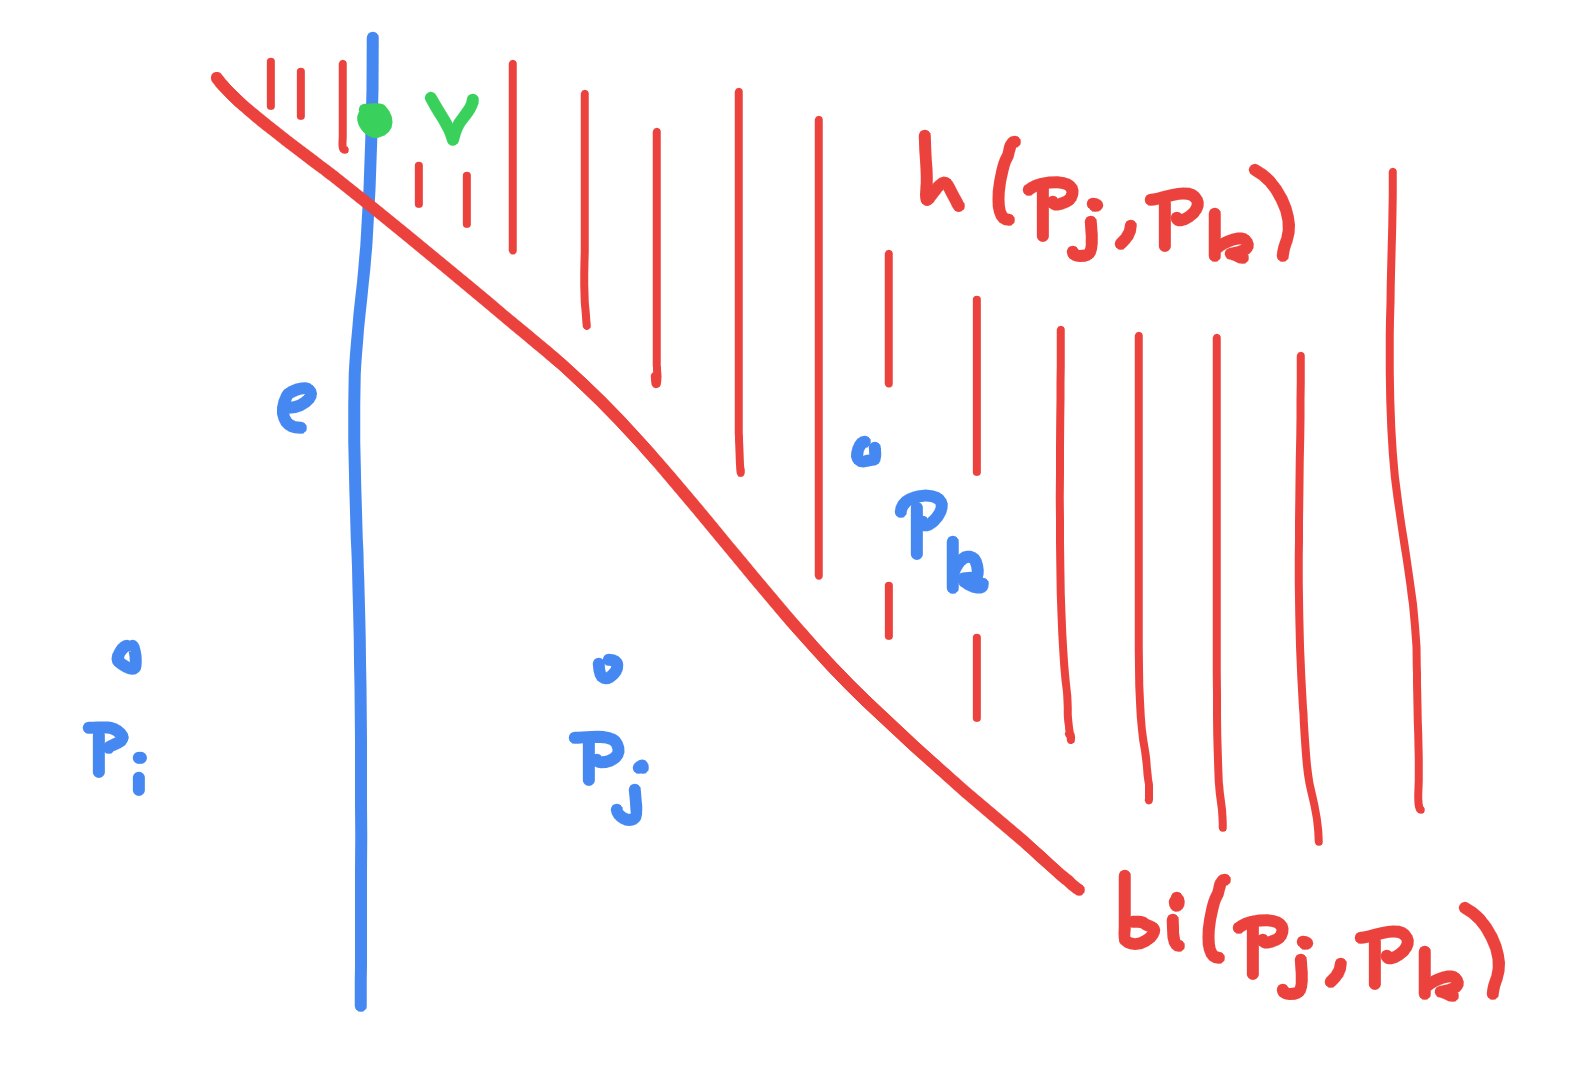
\includegraphics[scale=0.22]{temp-fig-4}
\]
We have that $v \in \partial\mathcal{V}(p_j)$ by definition of $e$. Now note that
\[
    \partial \mathcal{V}(p_j) = \partial \para{\bigcap_{a \ne j} h(p_j, p_a)} \subset^{\footnotemark} \bigcup_{a \ne j} \partial h(p_j, p_a) = \bigcup_{a \ne j} \bi(p_j, p_a).
\]
\footnotetext{Here we used that $\partial(A \cap B) \subset \partial A \cup \partial B$, a proof is here: \url{https://proofwiki.org/wiki/Boundary_of_Intersection_is_Subset_of_Union_of_Boundaries} \todo{Remove this footnote and add the result to some topology appendix}}As $v \in h(p_k, p_j)$ we have that $\dist(v, p_k) < \dist(v, p_j)$, hence $v \not\in \bi(p_j, p_k)$, so $v \not\in \partial{V}(v_j)$ by the above characterization of $\partial \mathcal{V}(p_j)$.
This is a contradiction, so $e$ can't be a full line. Now we show that $\VorG(P)$ is connected. Assume for the sake of a contradiction that $\VorG(P)$ is not connected. Then there exists a $\partial \mathcal{V}(p_i)$ which is not path connected. This can only happen if $\partial \mathcal{V}(p_i)$ consists of two parallel lines \todo{Why?}. This contradicts the fact that $\VorG(P)$ contains no lines. Thus $\VorG(P)$ is connected.
\end{proof}

Finally, we show that that the complexity of the vertices and edges is $\mathcal{O}(n)$:
\begin{thm}
For $n \geq 3$, the number of vertices in $\VorG(P)$ is at most $2n - 5$ and the number of edges is at most $3n - 6$.
\end{thm}
\begin{proof}
If the points in $P$ are collinear, then Theorem \ref{prop:structureofentirevoronoidiagram} implies the claim. Now assume that the points in $P$ are not collinear. As a first preprocessing step, we start by transforming $\VorG(P)$ into an actual plane graph, as some of the edges in $\VorG(P)$ may be half-lines. Let $v_1, \ldots, v_k$ denote the vertices of $\VorG(P)$. Let $p = \tfrac{1}{k}(v_1 + v_2 + \cdots + v_k) \in \R^2$ and let
\[
    r = 1 + \max\curly{\dist(p, v_1), \dist(p, v_2), \ldots, \dist(p, v_k)}.
\]
Then let $B_r(p) \subset \R^2$ denote the open ball with center $p$ and radius $r$. We have that $B_r(p)$ contains every vertex $v_i$ and that every half-line edge $e$ of $\VorG(P)$ intersects $\partial B_r(p)$ exactly once. Now define $v_{\infty} \in \R^2$ as any point in $\R^2 \setminus B_r(p)$ and transform every half-line edge $e$ into a path with finite length by connecting the half-lines to the point $v_{\infty}$. This is possible since $\R^2 \setminus B_p(r)$ only contains these half-lines, and every half-line is pointing in a unique direction so we may then transform the half-lines in order by starting with those which are closest to $v_{\infty}$. An example of this construction is given here:
\[
    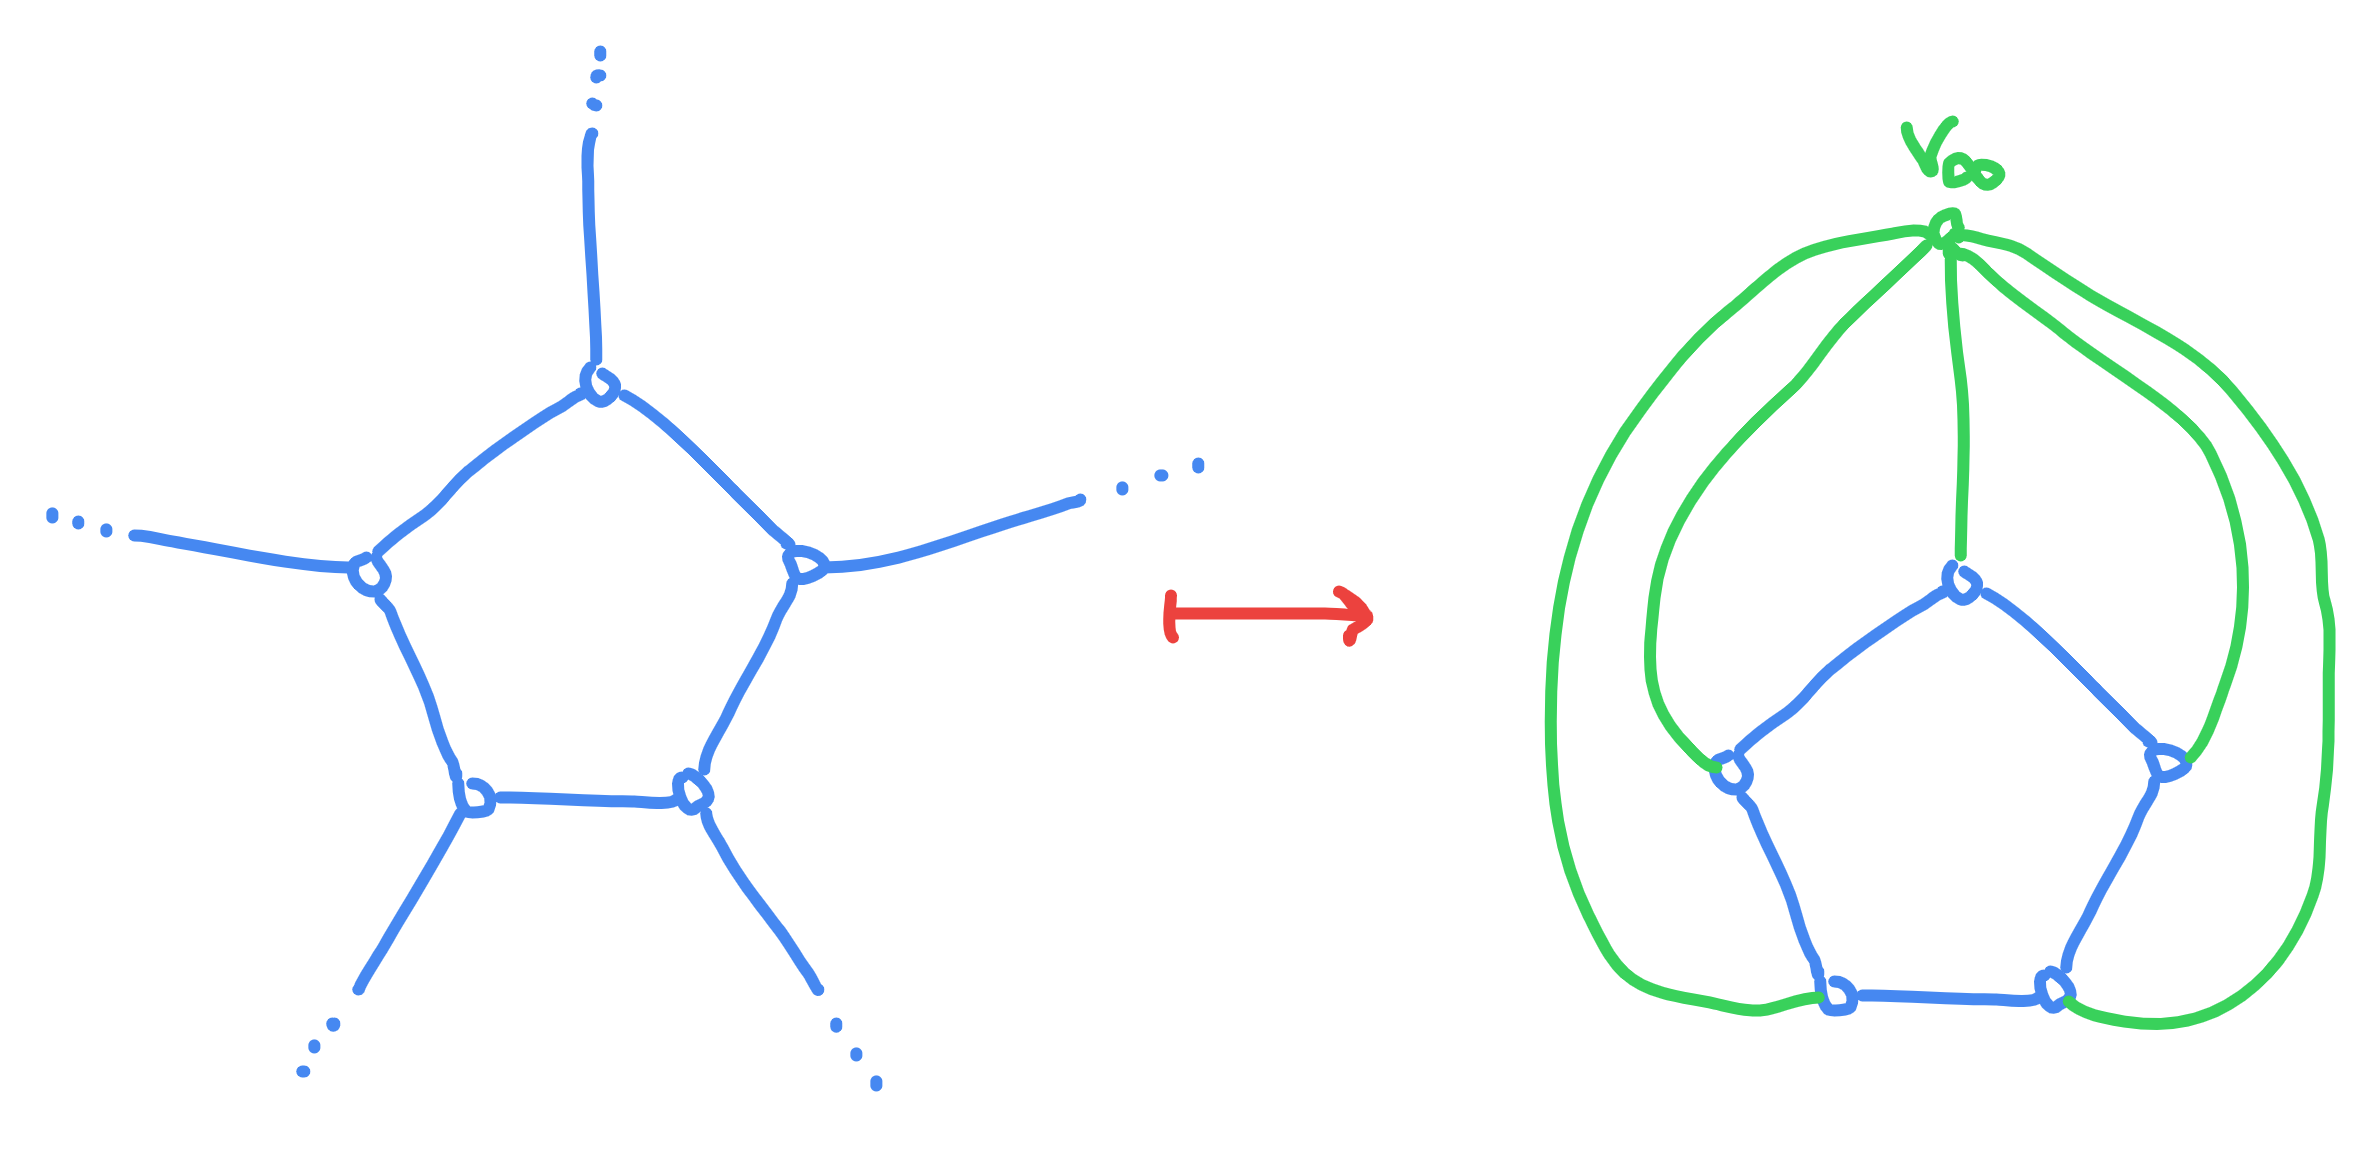
\includegraphics[scale=0.2]{temp-fig-5}
\]
In this way we can turn $\VorG(P)$ into a planar graph. For a planar graph $G$, Euler's formula\footnote{\todo{Add a reference and/or proof of Euler's formula in some topology appendix}} states that
\begin{equation} \label{eq:eulerformulainproof}
    V - E + F = 2,
\end{equation}
where $V$ is the number of vertices, $E$ is the number of edges and $F$ is the number of faces of $G$. Let $n_v$ denote the number of vertices of the original $\VorG(P)$, and let $n_e$ denote the number of edges. In our modification, we only added a single vertex, so by plugging into (\ref{eq:eulerformulainproof}) we obtain the following relationship:
\[
    (n_v + 1) - n_e + n = 2.
\]
Note that $n$ is the number of faces, since we have a Voronoi cell for each point in $P$. \todo{Finish}
\end{proof}

In the next section we will present an algorithm which computes $\Vor(P)$ in $\mathcal{O}(n \log n)$ time. This is actually optimal, as we can use a Voronoi diagram for sorting:
\begin{thm} \label{thm:voronoicansort}
We can't do better than $\mathcal{O}(n \log n)$.
\end{thm}
\begin{proof}
Let $A = \curly{a_1, a_2, \ldots, a_n} \subset \R$. Now assume we have used an algorithm to compute a Voronoi diagram of the points
\[
    P = \curly{(a_1, 0), (a_2, 0), \ldots, (a_n, 0)}.
\]
We obtain a diagram which looks similar to this:
\[
    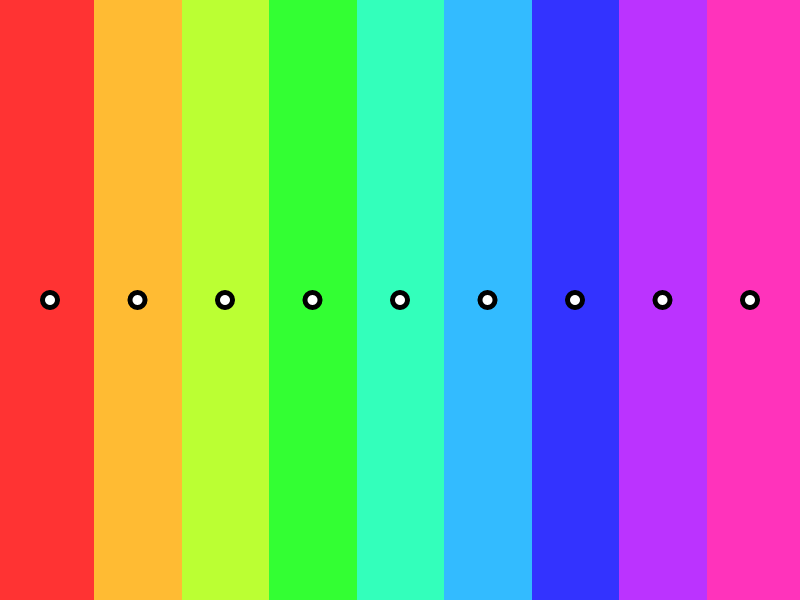
\includegraphics[scale=0.2]{voronoi-sorting}
\]
We assume without loss of generality that the algorithm outputs a DCEL $\Delta$ of $\Vor(P)$. Assume that the $\textsf{edge}$ pointer of every face of $\Delta$ points to the edge to the right of the face, and that the $\textsf{face}$ pointer of every edge of $\Delta$ points to the face to the right. Let $F_i$ be the face in $\Delta$ which contains the point $(0, a_i)$. Let $\ell \in \N$ such that $a_{\ell} < a_i$ for all $i \ne \ell$. Let $b_1 = a_{\ell}$ and if $b_i = a_{j}$ and $i < n$ then define $b_{i+1} = a_k$ where $k$ comes from $F_{j}\textsf{.edge.face} = F_k$. Then $(b_1, b_2, \ldots, b_n)$ is the elements of $A$ in sorted order. This means that we can use the Voronoi diagram to sort, which proves the theorem.
\end{proof}

\todo{The statement of the above theorem is temporary. I originally phrased it like so: ``The optimal worst-case running time for computing $\Vor(P)$ is $\Omega(n \log n)$.'' What is the proper terminology here?}